\section{Node Fingerprint} \label{PingLoad}
In this section, we propose an attack named ``PingLoad''\footnote{Stands for `PINGing payLoad''.} which allows an adversary to actively fingerprint applications running on different nodes, and later use this information to identify an application running on a specific node.

\subsection{The PingLoad Attack}

In \Cref{Sec:DistinguishDevice}  we mentioned the fact that processor occupied by other tasks may prolong the PRI.  \Cref{PingloadExample} illustrates such an example.

\AddFigure{fig/PINGLOAD_Session.png}{PRI prolonged by Sensor Reading}{PingloadExample}

\Cref{PingloadExample} illustrates an example where the PING Request is received when the node is processing a sensor reading. In this example, the measured PRI would include part of  sensor reading plus the actual time required for processing the PING request.

The PingLoad attack exploits the facts that:
\begin{itemize}
	%Routine application
	\item Typically nodes in WSN applications perform routine operations, e.g. collect the temperature  information for every 10 seconds, etc. 
	%Low performance
	\item The performance of the devices are low such that the difference in PRIs can be observed in the network traffic. As a counter example, the differences in PRIs on a desktop machine would be too small to be observed.
	%Different PRIs
	\item PRI prolongs differently when the processor is occupied by different tasks.
\end{itemize}

%How the attack works.
Therefore when sending a large amount of PING packets to different node running different applications, those prolonged PRIs would show distinctive distributions for different nodes performing different operations. \Cref{PingLoadTheory} illustrates an example that reading temperature sensor and ALS prolongs PRIs differently. 

\begin{figure}[ht!]
	\center
	\begin{subfigure}{0.8\textwidth}
	{
		\center
		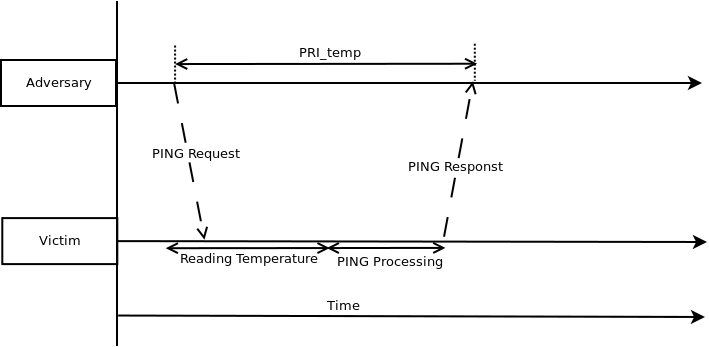
\includegraphics[width=\textwidth]{fig/PingLoad_temperature.png}
	}
	\subcaption{PRI when reading temperature sensor}
	\end{subfigure}
	\begin{subfigure}{0.8\textwidth}
	{
		\center
		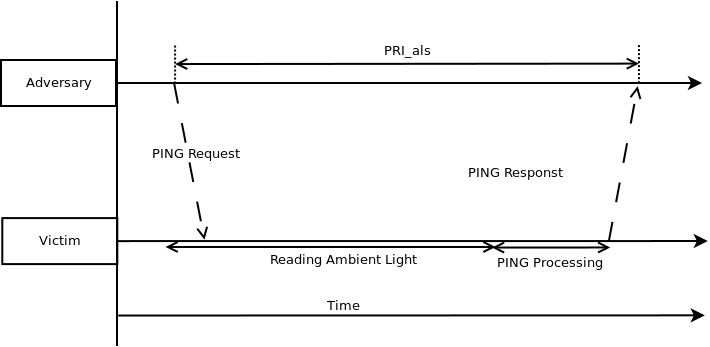
\includegraphics[width=\textwidth]{fig/PingLoad_als.png}
		\subcaption{PRI when reading Ambient Light Sensor(ALS)}
	}
	\end{subfigure}
	\caption{An example of reading temperature and ALS sensor results into different PRI.}
	\label{PingLoadTheory}
\end{figure}

The PingLoad attack hence uses such prolonged PRI distributions as fingerprints to different applications, matching an unknown application to known applications by finding  the statistically most similar PRI distribution. To be more specifically, the attack is described using a ``closed world'' setting with the following steps:

\begin{description}
	\item[Profiling]
	The first step requires the adversary to have the pre-knowledge of $n$ candidate applications, denote as $\mathbb{A} = \{A_1, A_2, ..., A_n\}$. The secret application to be identified, denote as $A_x$, is included in the set, such that $A_x \in \mathbb{A}$ where $x$ is unknown to the adversary.
	
	To fingerprint the applications, the adversary collects PRIs for each application in $\mathbb{A}$. We denote the profiled traces as:
	\begin{equation}
		\mathbb{T}_p = \{T_1, T_2, ..., T_n\}
	\end{equation}
where each $T_i$ is collected by repetitively sending PING request to a node running application $A_i$. Each trace $T_i$ contains multiple PRIs, denote as:
	\begin{equation}
		T_i = \{PRI^i_1, PRI^i_2, ..., PRI^i_{m_i}\} \text{ for } i \in [1,n]
	\end{equation}
	where $m_i$ is the number of PRIs in $T_i$.

	\item[Collecting Trace]
	To identify the secret application $A_x$, the adversary collects the PRI trace by sending PING requests to the node running $A_x$. We denote this collected trace as:
	\begin{equation}
		T_x = \{ PRI^x_1, PRI^x_2, ..., PRI^x_{m_x}\} % PRI_^x_1, $%PRI^x_2, ..., PRI^x_{m_x}\}$.
	\end{equation}
	
	\item[Matching Fingerprint]
	The first step of matching fingerprint is to filter out the PRIs those are affected by operations performed by the applications. In practice, a threshold $t$ can be observed from the traces. For example, for those PRIs of CC2538 we have shown in \Cref{PRIs}, $11$ms is a reasonable threshold as most PRIs are within the range of $[9,10.5]$(ms) for this device.
	Given the threshold $t$, we filter each traces in $\mathbb{T}$ by keeping only PRIs above the threshold:
	\begin{eqnarray}
		&\mathbb{T}^{\prime}_{p} &= \{ T^{\prime}_1, T^{\prime}_2, ..., T^{\prime}_n\} \\
		&T^{\prime}_{i} &= \{v | v > t, v \in T_i\} \text{ for } i \in [1,n]
	\end{eqnarray}
	We also filter the target trace using the same threshold:
	\begin{equation}
		T^{\prime}_x =  \{v | v > t, v \in T_x\}
	\end{equation}
	
	The adversary then searches $T^{\prime}_* \in \mathbb{T}^{`}_p$ that is statistically most similar to $T^{\prime}_x$. One way to do this is to use Kolmogorov-Smirniov Distance (KS-distance) as a measurement of statistical similarity and outputs the one with the minimum value, i.e. to search $T^{\prime}_*$ such that:
	\begin{equation}
		KSD( T^{\prime}_*, T^{\prime}_x) = min(\{KSD(T^{\prime}_i, T^{\prime}_x), i \in [1,n]\})
	\end{equation}
	where $KSD(X, Y)$ represents the KS-distance between two distributions $X$ and $Y$.
	
	Since $T^{\prime}_*$ is statistically most similar to $T^{\prime}_x$, the adversary outputs $A_*$ that corresponds to $T^{\prime}_*$ as the guess of $A_x$.
\end{description}

\subsection{Experiment}

We used 10 applications to test the PingLoad attack:
\begin{itemize}
	\item The \textbf{powertrace} example in Contiki source code which records the power consumption of the node.
	\item The \textbf{broadcast} example in Contiki source code which broadcasts the string ``Test'' periodically.
	\item The \textbf{sensorpayload} application family we developed. These applications periodically encrypt some sensor readings and send them back to the network root. We developped $8$ sensorpayload applications corresponding to $8$ different combinations of temperature, light and voltage sensors.
\end{itemize}

We  ran all applications on a CC2538 device. The PING requests are sent from a Linux host using ``ping6 -s 0 -i 0.4'', i.e. no user defined data and with interval of $0.4$ second. The frequency of PING is configured to such value to maximise the speed of collection without flooding the node.

For each application, we collected $2$ groups of packets dumps (pcapng files), with each dump consists of $200000$ packets. Traces of nearly $7000$ PRIs are extracted from each dump. Applying the empirical $11$ms threshold for CC2538, we gathered roughly 1000 PRIs from each filtered trace those are prolonged by the application. \Cref{PingLoadApps} summarises the data we used in the experiment.

For each of the 20 traces, we computed the KS-distances against all other 19 traces, with only one collected on the same application. \Cref{ksdistances} shows the result of KS-distances. Referring the indexes of minimum KS-distances in each row in \Cref{ksdistances} to \Cref{PingLoadApps}, our experiment reported 13 out of 20 ($65$\%) cases have successfully matched to the correct applications in our setting.

\paragraph{Analysis of Effectiveness}

Assume the traces does not contain any information of their corresponding application, i.e. each trace is uniformly randomly matched to one in the other 19 traces. The theoretical probability $P_0$ of having 13 out of 20 traces correctly matched is:
\begin{equation*}
P_0 = C^{13}_{20} (\frac{1}{19})^{13} (\frac{18}{19})^{7} \approx 1.262 * 10^{-12} \leq 0.01
\end{equation*}

Therefore we reject the hypothesis and conclude that the traces contain information of the applications.